\documentclass[11pt]{beamer}
\usetheme{Singapore}

\usepackage[utf8]{inputenc}
\usepackage[english]{babel}
\usepackage{amsmath}
\usepackage{amsfonts}
\usepackage{amssymb}
\usepackage{graphicx}
\usepackage{indentfirst}
\usepackage{ragged2e}
\usepackage[section]{placeins}
\usepackage{amssymb, amsfonts, amsmath,bm} % Math symbols, fonts,
\usepackage{mathptmx} 
\usepackage{subcaption}
\usepackage{caption}
\usepackage{breqn}
\usepackage{threeparttable} %
\captionsetup[figure]{textfont=scriptsize, labelfont=scriptsize}
\captionsetup[subfigure]{font=scriptsize, labelfont=scriptsize}
\DeclareMathOperator*{\argmin}{arg\,min} 
\DeclareMathOperator*{\argmax}{arg\,max} 
\DeclareMathOperator*{\arginf}{arg\,inf} 
\DeclareMathOperator*{\argsup}{arg\,sup}
\addtobeamertemplate{navigation symbols}{}{%
	\usebeamerfont{footline}%
	\usebeamercolor[fg]{footline}%
	\hspace{1em}%
	\insertframenumber/\inserttotalframenumber
}
%\author{}
%\title{}
%\subtitle{}
%\logo{}
%\institute{}
%\date{}
%\subject{}
%\setbeamercovered{transparent}
\usepackage[authoryear,round ]{natbib}
%\setcitestyle{numbers,open={[},close={]}}
\bibliographystyle{plainnat}
%\renewcommand{\labelitemii}{*}
\author{Aiden Huffman, Ben Sloman, Jinniao Qiu, Syeda Ali, Tony Ware, Wenning Wei, Zuming Sun and Yilan Luo\\
 (Project Coordinator: Michael Morgan)
}
\title{Stochastic Modeling of Oil and Gas Production
}


\begin{document}


%%%%%%%%%%%%%%%%%%%%%%%%%%%%%%%%%%%%%%%%%
%%%%%%%%%% Content starts here %%%%%%%%%%
%%%%%%%%%%%%%%%%%%%%%%%%%%%%%%%%%%%%%%%%%
\upshape
\maketitle
\begin{frame}
	\tableofcontents
\end{frame}


%%%%%%%%%%%%%%%%%%%%%%%%%%%%%%%%%%%%%%%%%%%%%%%%%%%%%%%%%%%%%%%%
\section{1.Introduction}
	\begin{frame}
    	\frametitle{Introduction}
        \framesubtitle{Montney Wells}
        \justifying
       \begin{itemize}
            \item Oil and gas operators in both British Columbia and Alberta are currently persuing development of the Montney formation.
            \item It is currently one of the top plays in North America, in terms of number of wells drilled per year, investment dollars spent and overall hydrocarbon production.
            \item It covers a geographical region of approximately 130,000km, with thickness between 100m-300m.
            \item Due to its thickness, much of the Montney can supported multiple layers of stack horizontal wells.
            \item The Montney holds approximately 449 Tcf of marketable natural gas.
         \end{itemize}
     \end{frame}

\begin{frame}
\begin{figure}
\begin{center}
\includegraphics[width=0.48\textwidth]{"montney_well".png} 
\caption{Montney Major Rock Types.}
\label{smooth}
\end{center}
\end{figure}
	\end{frame}	
	
\begin{frame}
	\frametitle{Introduction}
    \framesubtitle{Background}
Many Challenges of the oil and gas industry subject to production uncertainty are as follows:
\begin{itemize}
\item Finding oil and gas reserves is highly unpredictable.
\item Productivity of an individual well change in random ways.
\item Very noisy data.
\item Market moves unexpectedly.
\item Future prices and interest rates are unknown.
\end{itemize}
\end{frame}

\begin{frame}
\frametitle{Introduction}
\framesubtitle{Motivation}
\begin{itemize}
\item In Industries we are interested in the mechanism of how uncertainties are treated as workload moves to reserves production development.
\item Basic ODE's cannot capture these uncertainties very well.
\item Stochastic models offers a methodology to better capture the uncertainties of the process. by treating some unknown parameters as random variables.  

\end{itemize}

\end{frame}
\begin{frame}

\frametitle{Introduction}
\framesubtitle{Goal}
\begin{itemize}
\item To model the unknown parameters as stochastic processes.
\item Solve the resulting stochastic differential equations.
\item Comparing our results with data from actual well to witness the performance.
\end{itemize}
\end{frame}


    \begin{frame}
		\frametitle{Introduction}
        \framesubtitle{Basic Definitions}
		\justifying
		\begin{itemize}
			\item Flow rate ($q$): The mount of gas produced per time unit for several consecutive period.
			\item Cumulative gas production ($Q$): $\int_{0}^{T}qdt $	
			\item Decline rate(D): $D=-\dfrac{1}{q}\frac{\Delta q}{\Delta t}$	
		\end{itemize}
	\end{frame}
\begin{frame}
\frametitle{Introduction}
\framesubtitle{Decline Curve Analysis}
\begin{itemize}
\item Use to estimate the production of a well, while original data is given.
\item Use to forecast the future performance of wells.
\item Production trends can be estimated using different differential equations, for example, Hyperbolic, Exponential etc.
\end{itemize}
\end{frame}
	\begin{frame}
		\frametitle{Introduction}
		\framesubtitle{Production Delcine Curve}
		\justifying
\begin{figure}
\begin{center}
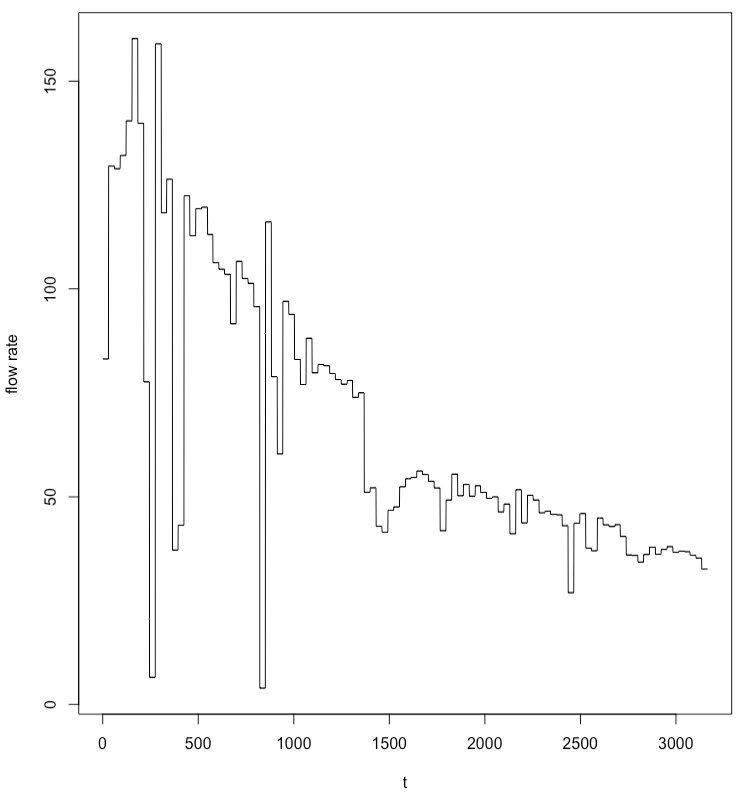
\includegraphics[width=0.6\textwidth  ]{decline} 
\caption{An example of decline curve of flow rate of gas. }\label{smooth}
\end{center}
\end{figure}
	\end{frame}		

\section{2.Modeling and Estimation}		
	\begin{frame}
		\frametitle{Modeling and Estimation}
		\framesubtitle{Data Description}
		\justifying
	\begin{figure}
\begin{center}
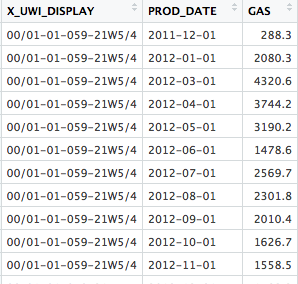
\includegraphics[width=0.6\textwidth  ]{data} 
\caption{An snapshot of dataset. }
\end{center}
\end{figure}	
	\end{frame}		
		
	\begin{frame}
		\frametitle{Modeling and Estimation}
		\framesubtitle{Common PDE models in Delcine Analysis}
		\justifying
\begin{figure}
\begin{center}
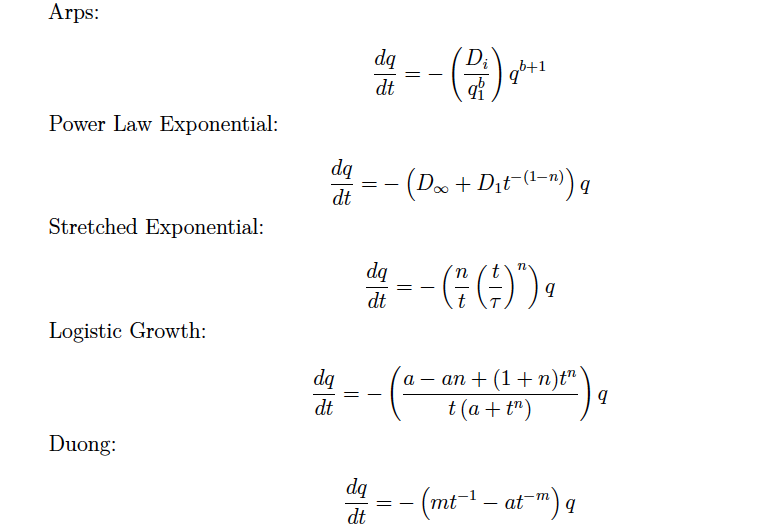
\includegraphics[width=0.8\textwidth  ]{model} 
\end{center}
\end{figure}
	\end{frame}		
				
	\begin{frame}
		\frametitle{Modeling and Estimation}
		\framesubtitle{Parameter Estimation of Classic PDE Models by LS}
	\begin{figure}
\begin{center}
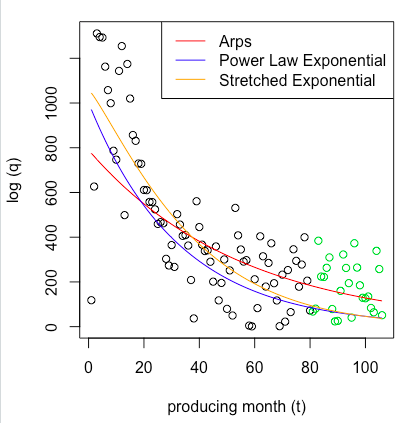
\includegraphics[width=0.65\textwidth  ]{arps} 

\end{center}
\end{figure}	
	\end{frame}		
				
	\begin{frame}
		\frametitle{Modeling and Estimation}
		\framesubtitle{Improved Power Law Exponential Model NO.1}
		\justifying
		\begin{itemize}
		\item Power law exponential model:
		\begin{equation}
		log(q)=log(q_0)-D_\infty t - Dt^n
		\end{equation}
		\item First, we assume $log(q_0)\sim m+\varepsilon N(0,1)$
		\item To generate the uncertainty in the model, we also add a Brownian Motion item with a scale parameter $\lambda$:
		$\lambda B_t$
		\item Therefore, the proposed model is:
		\begin{equation}
		log(q)=m+\varepsilon N(0,1)-D_\infty - Dt^n+\lambda B_t
		\end{equation}
		\end{itemize}		
			\end{frame}		


	\begin{frame}
		\frametitle{Modeling and Estimation}
		\framesubtitle{Improved Power Law Exponential Model NO.2}
		\justifying
		\begin{itemize}
		\item Since the $B_t\sim N(0,\sqrt{t})$ and the well is always run for a long time, the fluctuation of model NO.1 is too large at the late time of well.
		\item We weight $B_t$ with $\dfrac{1}{1+t}$
		\item Therefore, the model change to:
		\begin{equation}
		log(q)=m+\varepsilon N(0,1)-D_\infty - Dt^n+\dfrac{\lambda B_t}{1+t}
		\end{equation}
		\end{itemize}		
	\end{frame}		
	
	\begin{frame}
		\frametitle{Modeling and Estimation}
		\framesubtitle{Estimation of Model NO.2}
		\justifying
		\begin{itemize}
		\item Then we estimate the parameters ($m,\varepsilon,D_\infty,D,n,\lambda$) in the model (by Maximum Likelihood)  minimizing
		\begin{eqnarray*}
		&\dfrac{1}{2}log(\varepsilon^22\pi)+\dfrac{(log(q_0)-m_0)^2}{2 \pi \varepsilon^2} \\
		&+\sum_{i=1}^N\left(\frac{1}{2}log\left(\frac{\lambda^22\pi}{(1+t_{i-1})^2}\right)+\dfrac{(log(q_{t_i})-log(q_{t_{i-1}})+D_\infty+Dt_i^n)^2}{\dfrac{2\pi\lambda^2}{(1+t_{i-1})^2}}\right)
		\end{eqnarray*}
		\end{itemize}		
	\end{frame}		
	
				
	\begin{frame}
		\frametitle{Modeling and Estimation}
		\framesubtitle{Estimation Result}
		\justifying
\begin{figure}
\begin{center}
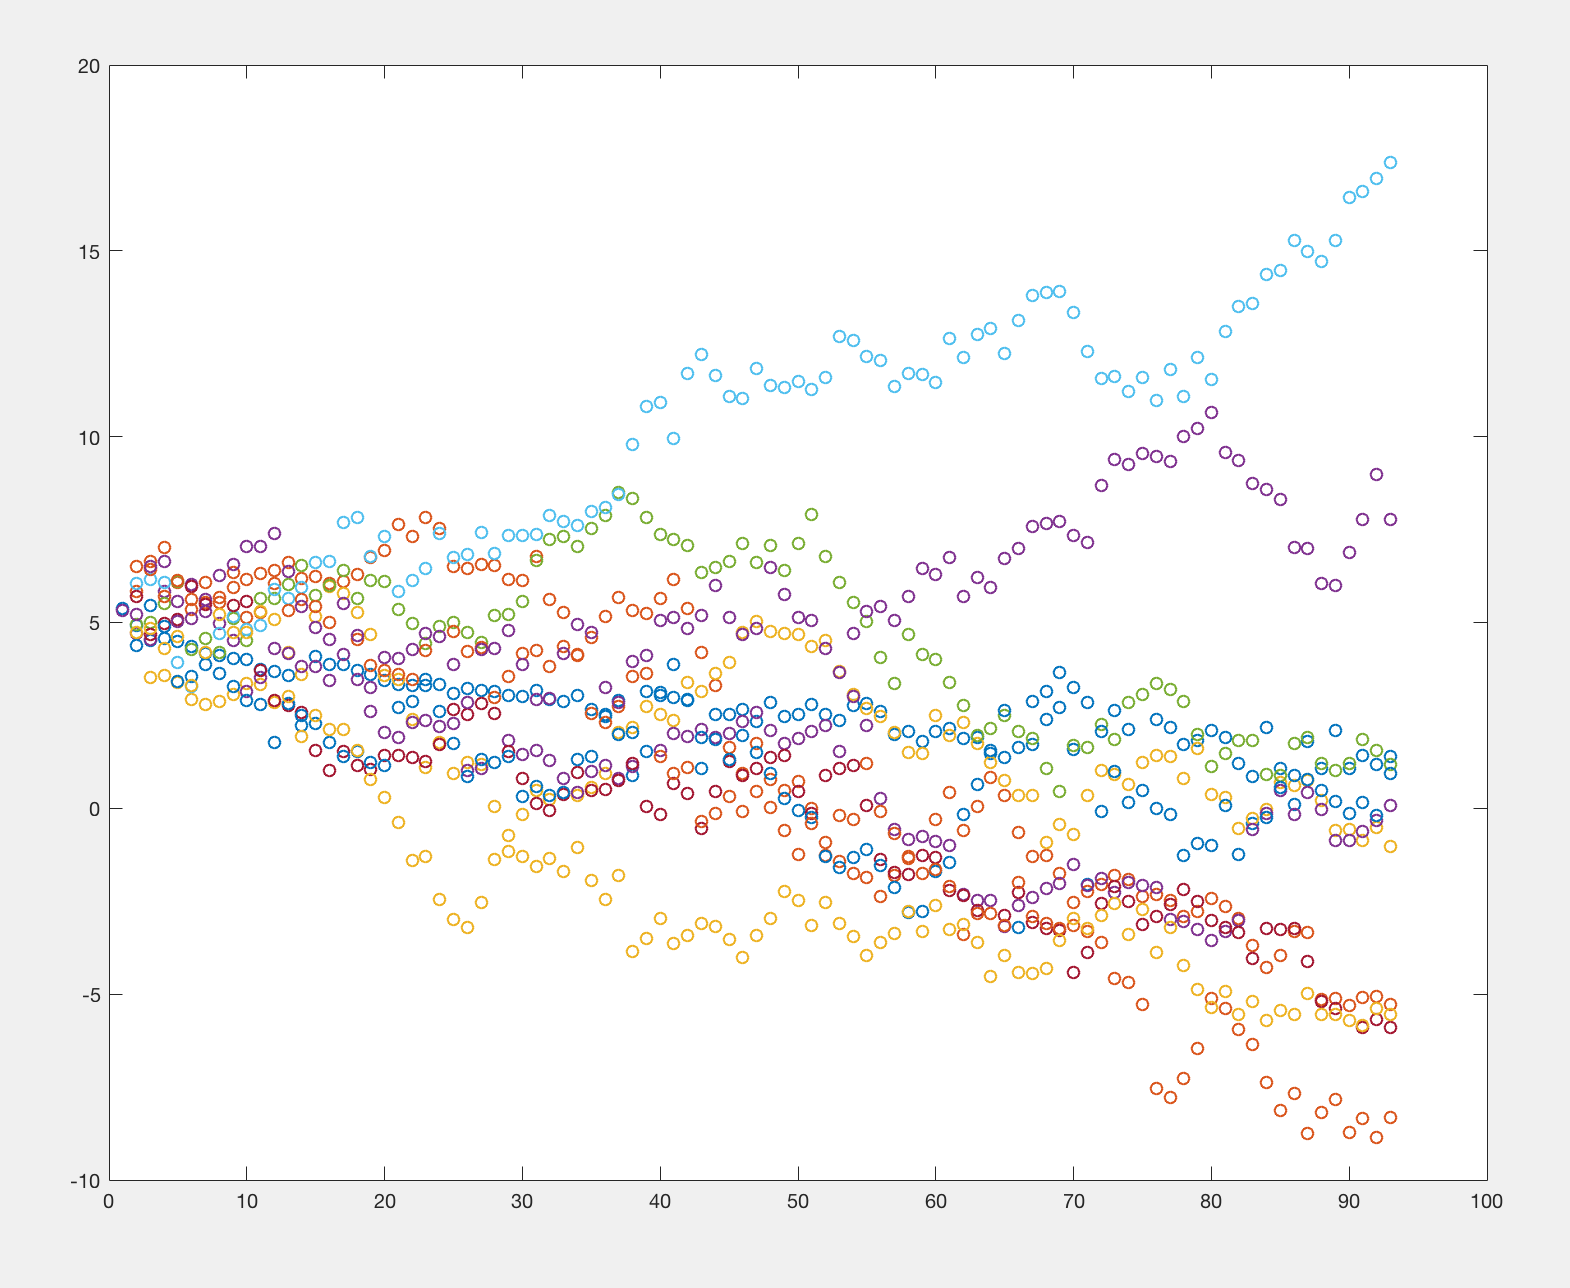
\includegraphics[width=0.8\textwidth  ]{like.PNG} 

\end{center}
\end{figure}
	\end{frame}		
	
				
	\begin{frame}
		\frametitle{Modeling and Estimation}
		\framesubtitle{Improved Power Law Exponential Model NO.3}
		\justifying
\begin{itemize}
		\item We improve the model
		\item Then the log-likelihood: find $(m_0,\varepsilon,\lambda,m,D,D_{\infty})$ minimizing
		\begin{eqnarray*}
		&\dfrac{1}{2}log(\varepsilon^22\pi)+\dfrac{(log(q_0)-m_0)^2}{2 \pi \varepsilon^2} \\
		&
		+\sum_{i=1}^N\left(\dfrac{1}{2}log(\frac{\lambda^22\pi}{(1+t_{i-1}^m)^2})+\dfrac{(log(q_{t_i})-log(q_{t_{i-1}})+D_\infty+Dt_{i-1}^n)^2}{\dfrac{2\pi\lambda^2}{(1+t^m_{i-1})^2}}\right)
		\end{eqnarray*}
		\end{itemize}		
	\end{frame}	
	
	
	\begin{frame}
		\frametitle{Modeling and Estimation}
		\framesubtitle{Improved Power Law Exponential Model NO.3}
		\justifying
	\begin{figure}
\begin{center}
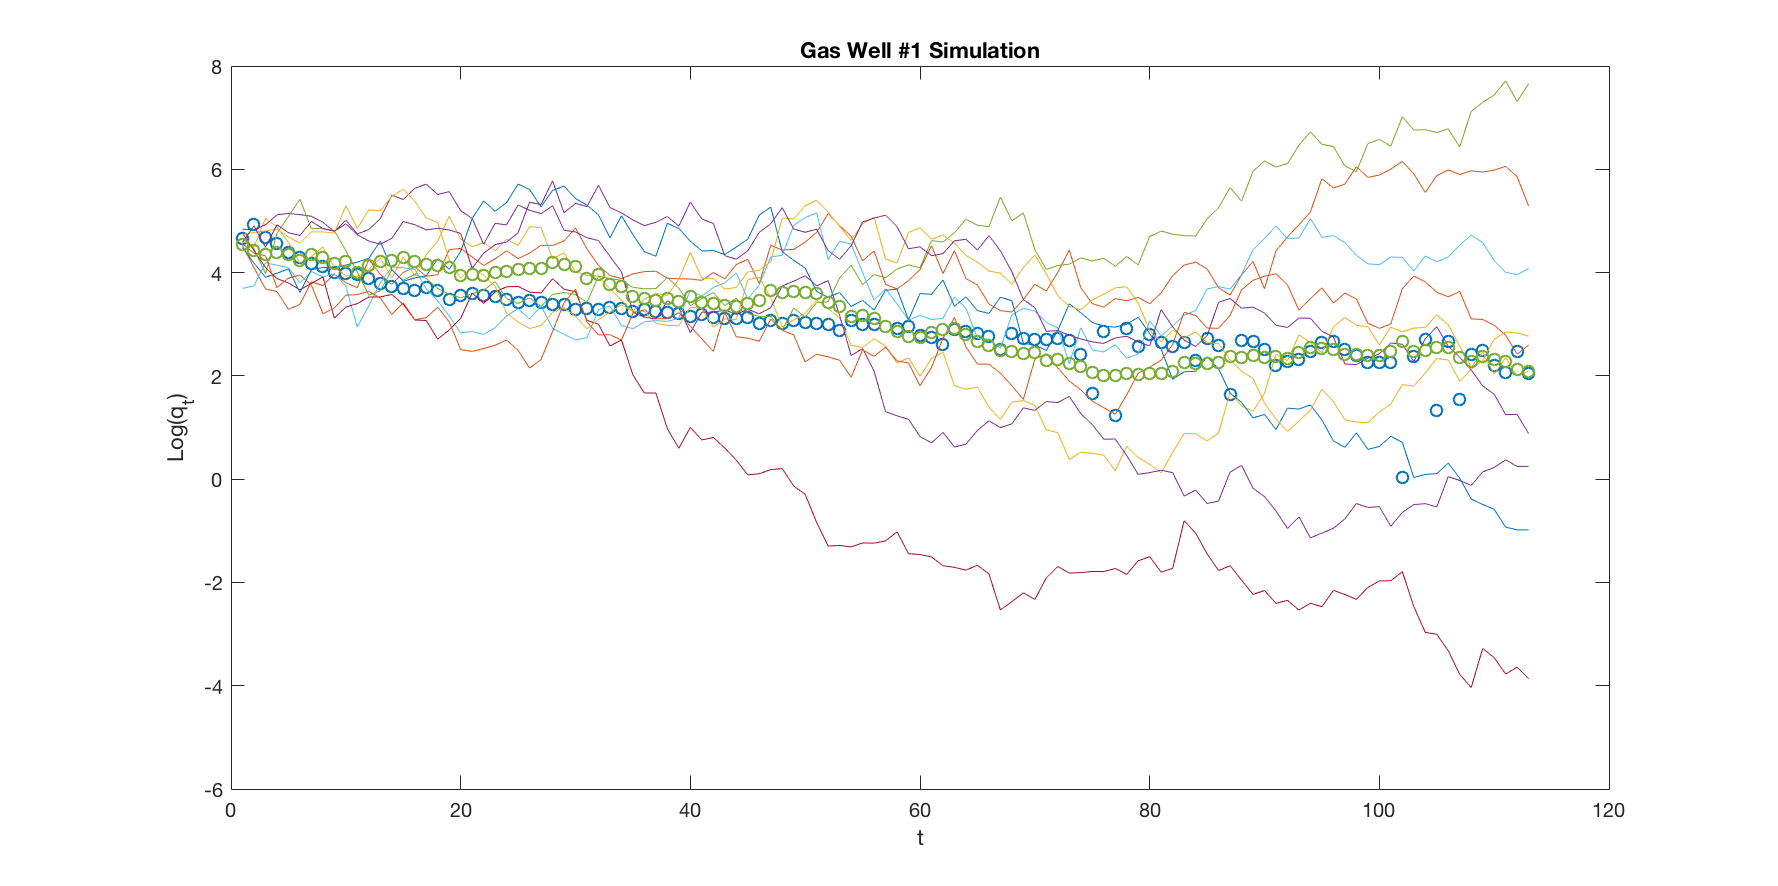
\includegraphics[width=1.1\textwidth  ]{intmodel} 

\end{center}
\end{figure}				
	\end{frame}	

	
	\begin{frame}
		\frametitle{Modeling and Estimation}
		\framesubtitle{Improved Power Law Exponential Model NO.3}
		\justifying
\begin{itemize}
		\item Improve the model
		\item Modify the log-likelihood: find $(m_0,\varepsilon=0,\lambda,m,D,D_{\infty})$ minimizing
		\begin{eqnarray*}
		%& |m_0-D_\infty t_i-Dt_i^n-log(q_i^{obs})| \\
		& \sum_{i=1}^Nlog(\dfrac{2\pi\lambda^2}{(1+t_i^m)^2})\\
		&+\sum_{i=1}^N(log(q_{t_i}-log(q_{t_{i-1}})+D_\infty+Dnt_i^{n-1})^2\dfrac{(1+t^m_{i-1})^2}{2\pi\lambda^2}\\
		&+\kappa\sum_{i=1}^N|m_0-D_\infty t_i-Dt_i^n-log(q_i^{obs})|
		\end{eqnarray*}
		\end{itemize}	
			\end{frame}	
	
\begin{frame}
	\frametitle{Modeling and Estimation}
	\framesubtitle{Improved Power Law Exponential Model NO.4}
	\justifying
\begin{figure}
\begin{center}
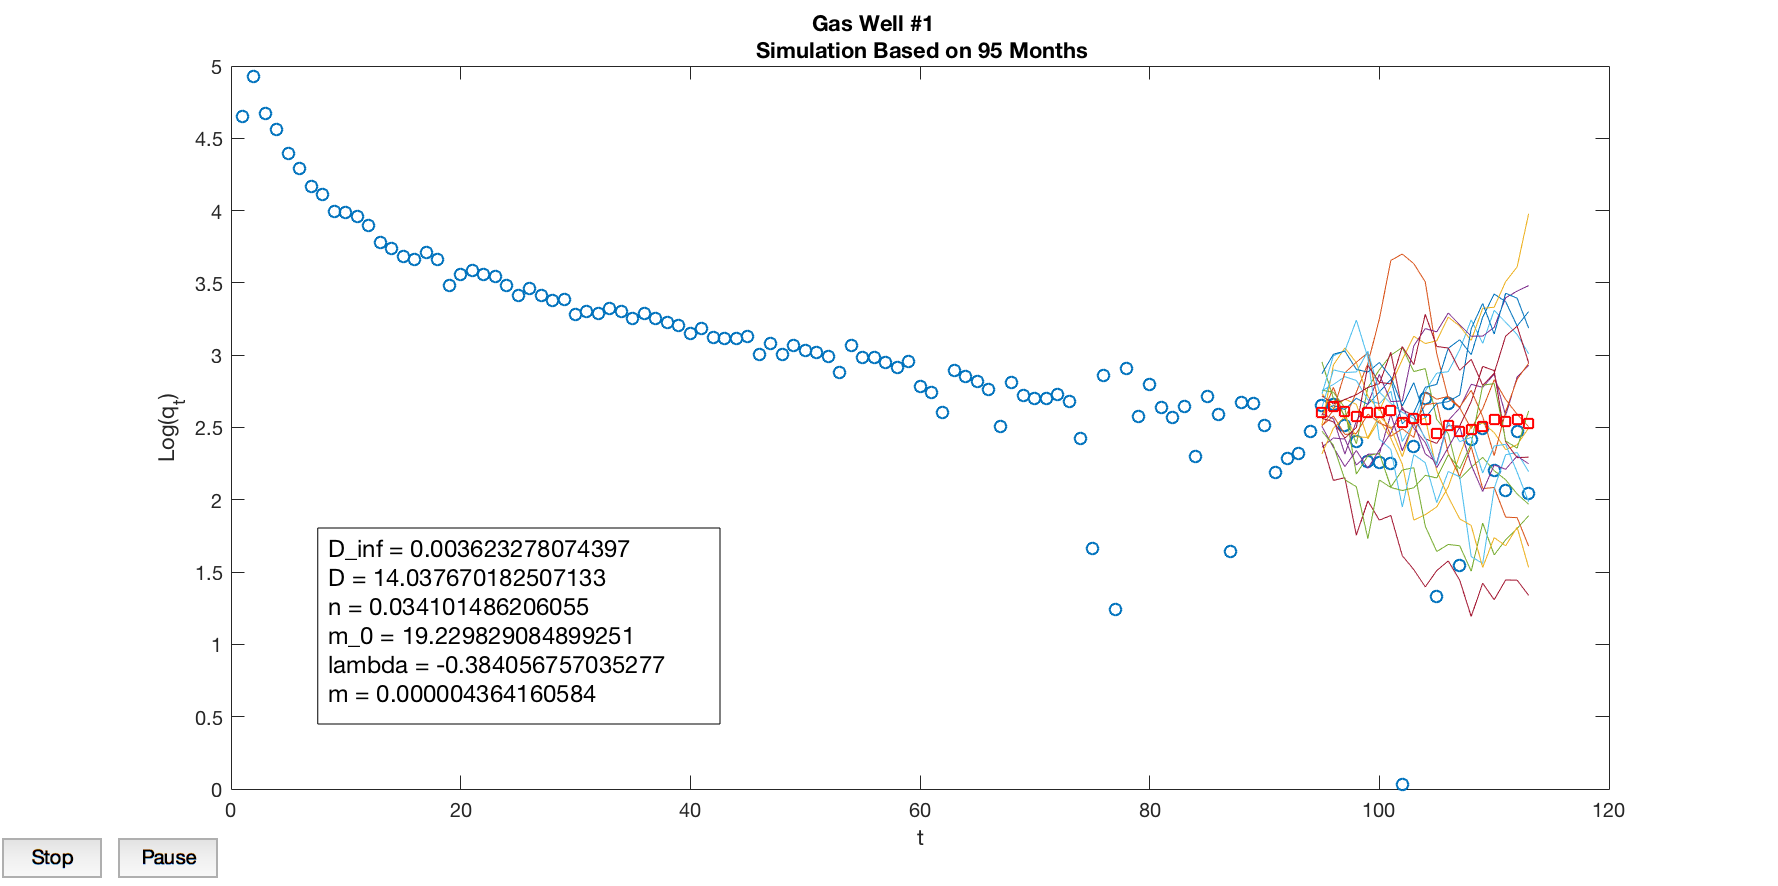
\includegraphics[width=1.1\textwidth  ]{well1} 
\end{center}
\end{figure}				
\end{frame}	

	\begin{frame}
		\frametitle{Modeling and Estimation}
		\framesubtitle{Improved Power Law Exponential Model NO.4}
		\justifying
\begin{itemize}
		\item Except Brownian Motion, we also consider the Poisson process to describe the uncertainty in the reality.
		\item Simply, we replace the Brownian Motion by a Poisson Process $N_t^{\alpha}$:
		\begin{equation}
		log(q)=m+\varepsilon N(0,1)-D_\infty - Dt^n+\lambda N_t^{\alpha}
		\end{equation}
		\item Then the least square norm: ($\varepsilon=0$): find $(m_0,\lambda,m,D,D_{\infty},\alpha)$ minimizing
		\begin{eqnarray*}
		%& |m_0-D_\infty t_i-Dt_i^n-log(q_i^{obs})| \\
%		& \sum_{i=1}^Nlog(\dfrac{2\pi\lambda^2}
%{(1+t_i^m)^2})\\
		&E\sum_{i=1}^N\left(\Delta log(q^{mod}_{t_i})-\Delta log(q^{obs}_{t_{i}}) \right)^2
		\\
		&
		+\kappa\sum_{i=0}^N \left(E log(q^{mod}_{t_i})- log(q^{obs}_{t_{i}}) \right)^2
		\end{eqnarray*}
		\end{itemize}	
			\end{frame}	
	
\begin{frame}
	\frametitle{Modeling and Estimation}
	\framesubtitle{Improved Power Law Exponential Model NO.4}
	\justifying
\begin{figure}
\begin{center}
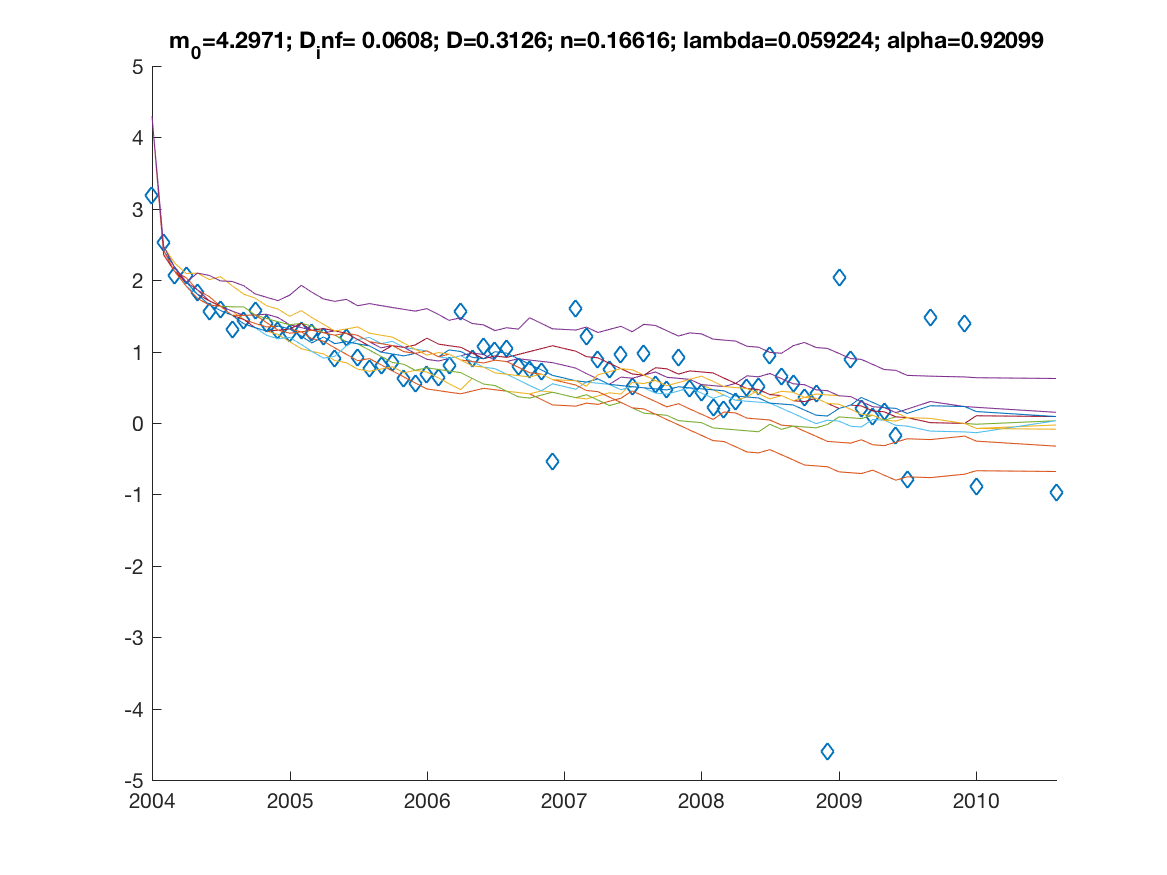
\includegraphics[width=0.9\textwidth  ]{AAplot_12} 
\end{center}
\end{figure}				
\end{frame}	

\begin{frame}
	\frametitle{Modeling and Estimation}
	\framesubtitle{Improved Power Law Exponential Model NO.4}
	\justifying
\begin{figure}
\begin{center}
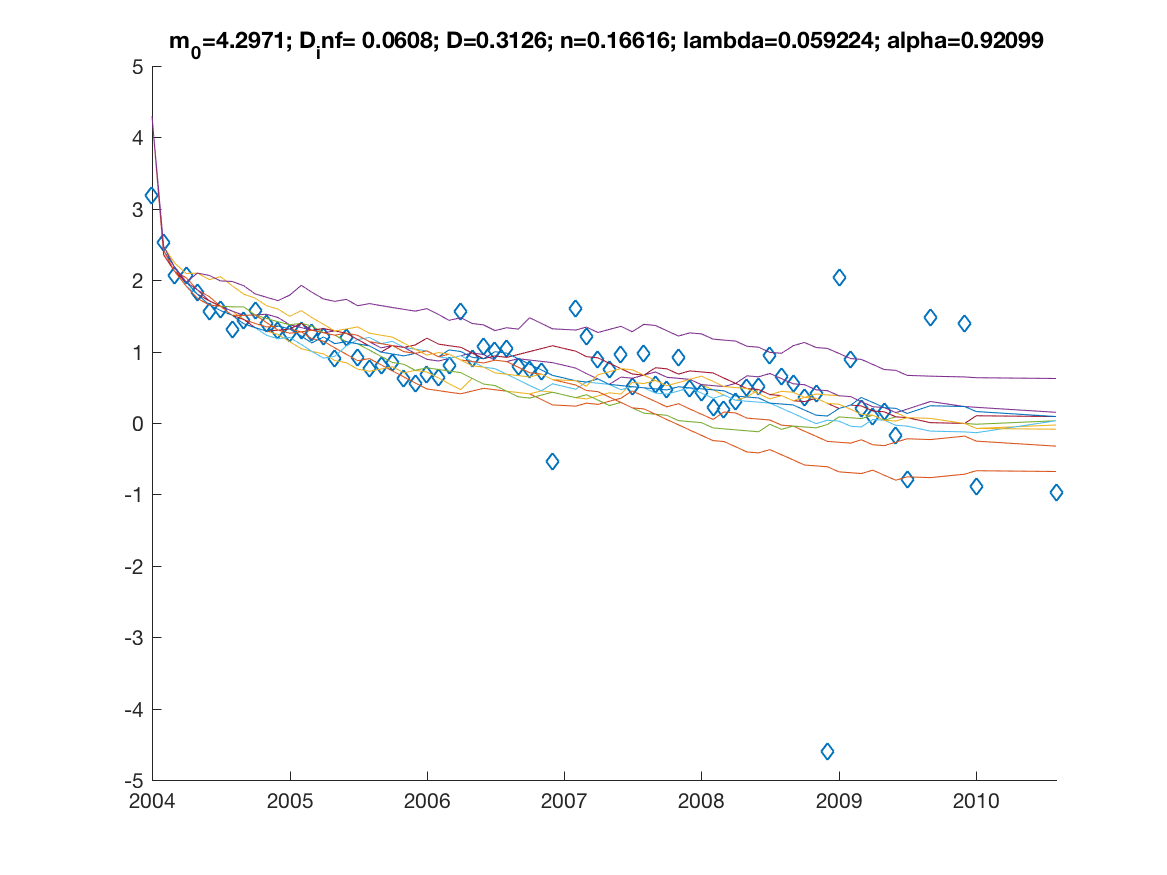
\includegraphics[width=0.9\textwidth  ]{AAplot_12} 
\end{center}
\end{figure}				
\end{frame}	

\begin{frame}
	\frametitle{Modeling and Estimation}
	\framesubtitle{Improved Power Law Exponential Model NO.4}
	\justifying
\begin{figure}
\begin{center}
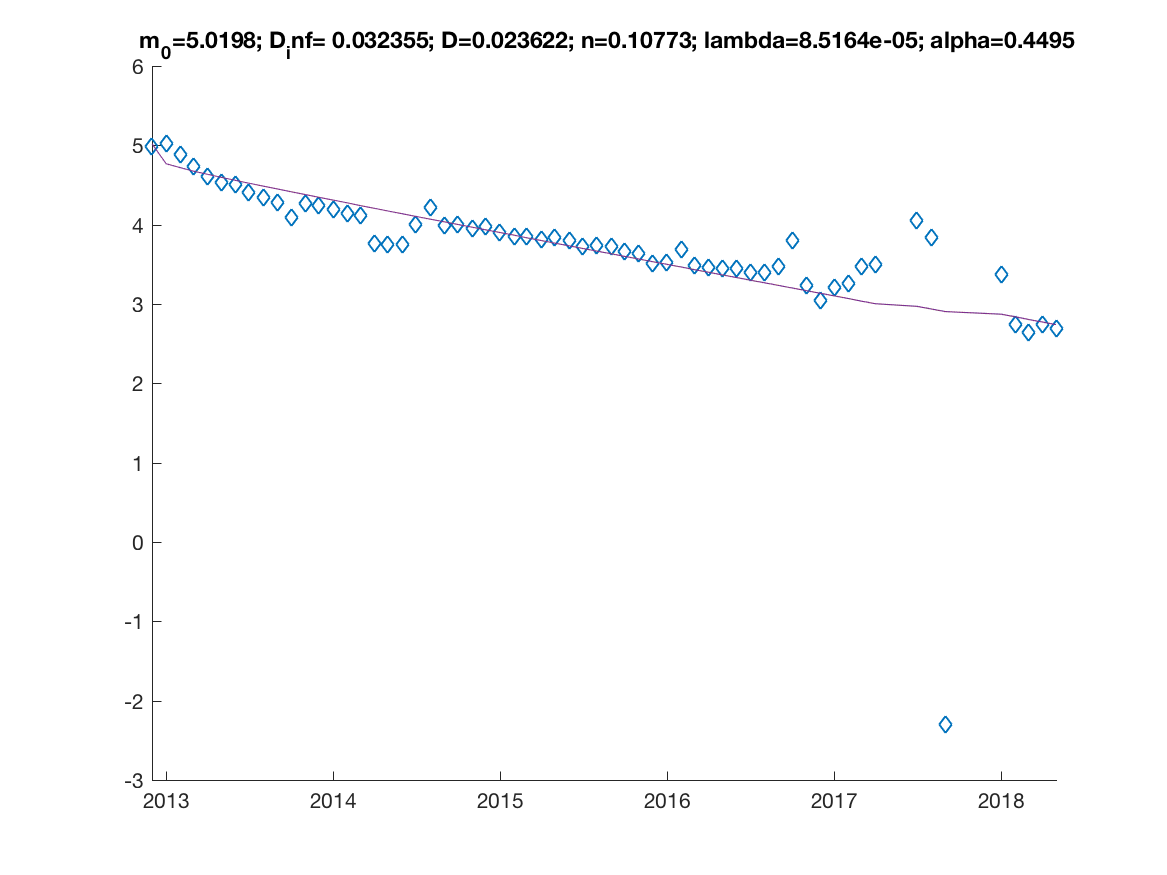
\includegraphics[width=0.9\textwidth  ]{AAplot_21} 
\end{center}
\end{figure}				
\end{frame}	

\begin{frame}
	\frametitle{Modeling and Estimation}
	\framesubtitle{Improved Power Law Exponential Model NO.4}
	\justifying
\begin{figure}
\begin{center}
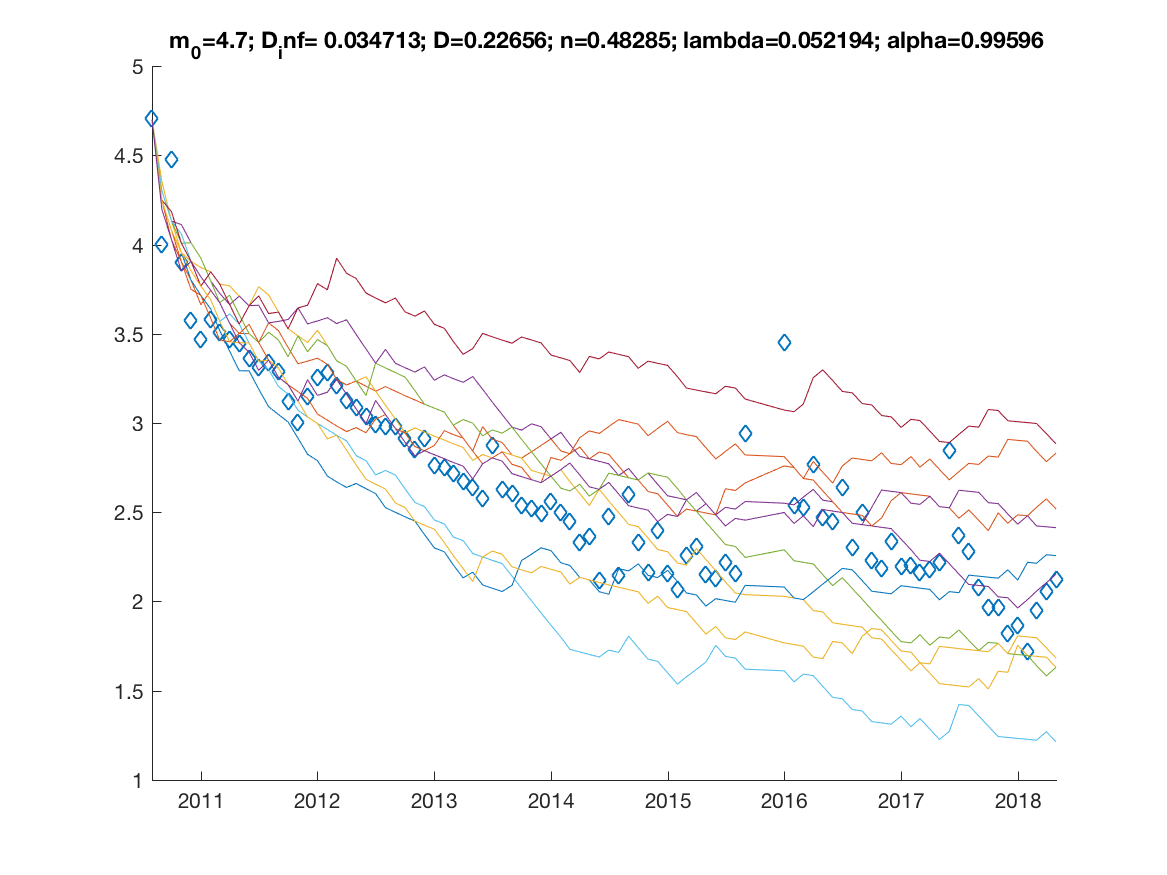
\includegraphics[width=0.9\textwidth  ]{AAplot_27} 
\end{center}
\end{figure}				
\end{frame}	

\begin{frame}
	\frametitle{Modeling and Estimation}
	\framesubtitle{Improved Power Law Exponential Model NO.4}
	\justifying
\begin{figure}
\begin{center}
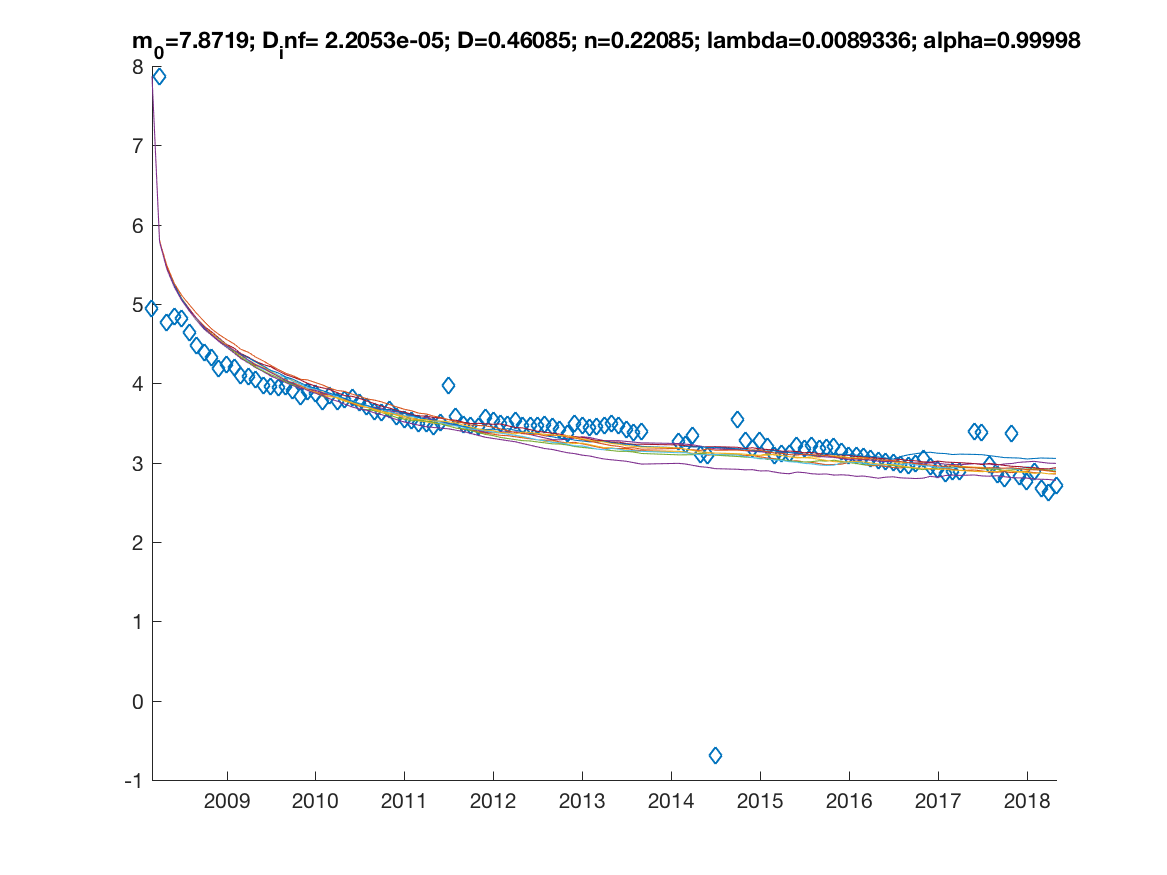
\includegraphics[width=0.9\textwidth  ]{AAplot_374} 
\end{center}
\end{figure}				
\end{frame}	

\begin{frame}
	\frametitle{Modeling and Estimation}
	\framesubtitle{Improved Power Law Exponential Model NO.4}
	\justifying
\begin{figure}
\begin{center}
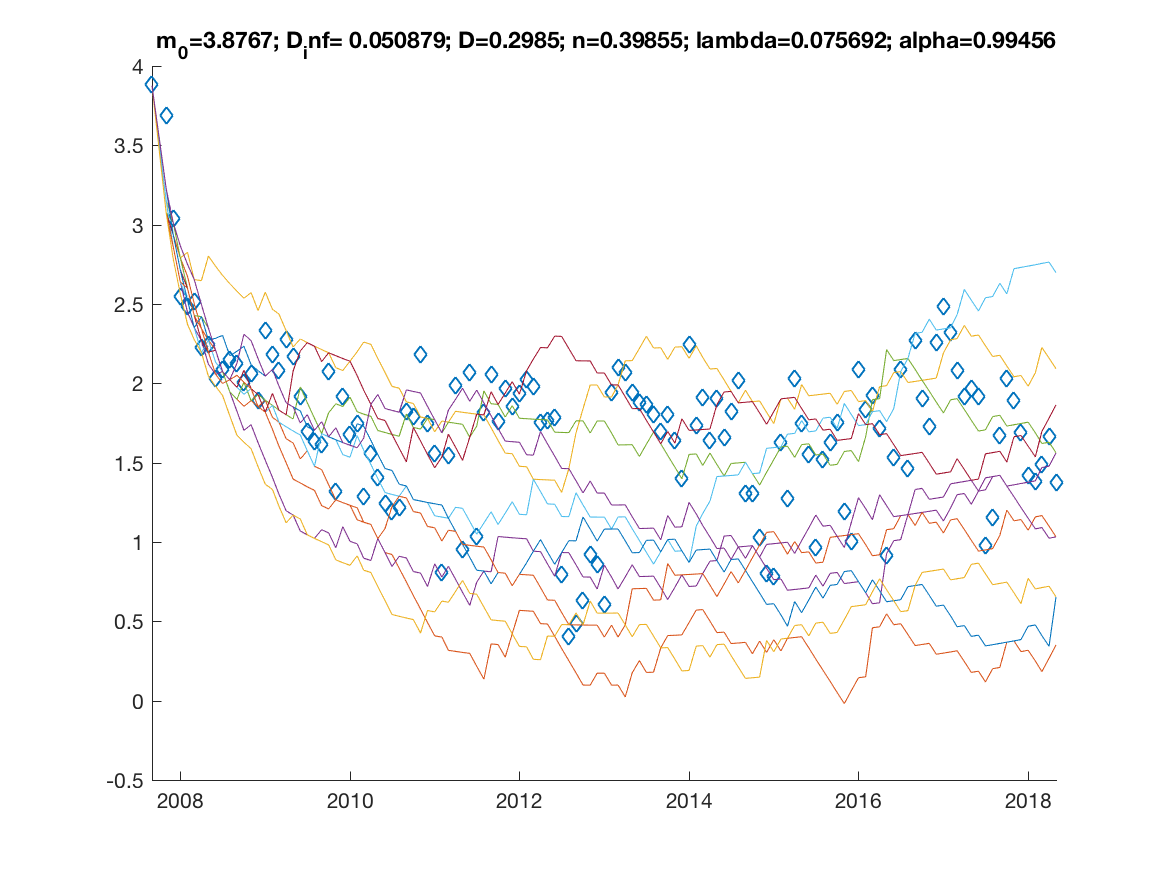
\includegraphics[width=0.9\textwidth  ]{AAplot_1153} 
\end{center}
\end{figure}				
\end{frame}	

\begin{frame}
	\frametitle{Modeling and Estimation}
	\framesubtitle{Improved Power Law Exponential Model NO.4}
	\justifying
\begin{figure}
\begin{center}
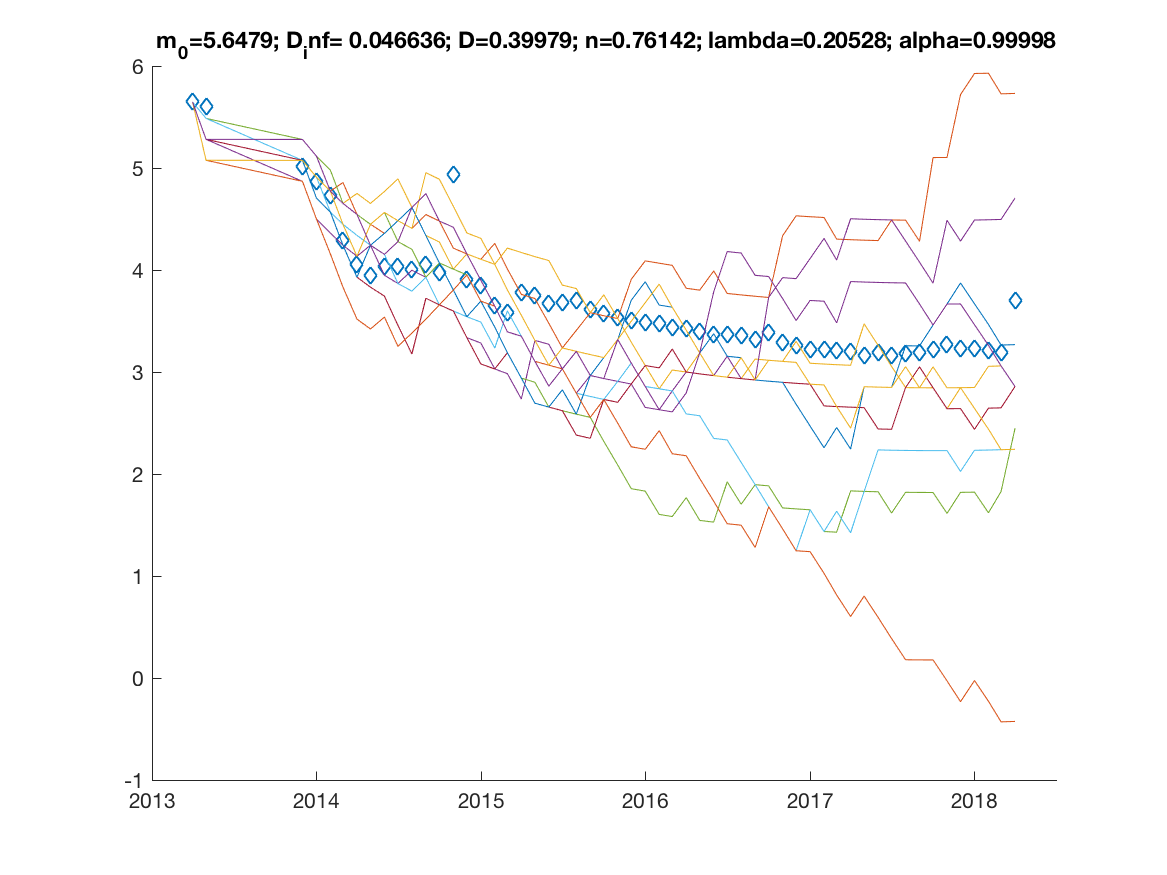
\includegraphics[width=0.9\textwidth  ]{BBplot_87} 
\end{center}
\end{figure}				
\end{frame}	

\begin{frame}
	\frametitle{Modeling and Estimation}
	\framesubtitle{Improved Power Law Exponential Model NO.4}
	\justifying
\begin{figure}
\begin{center}
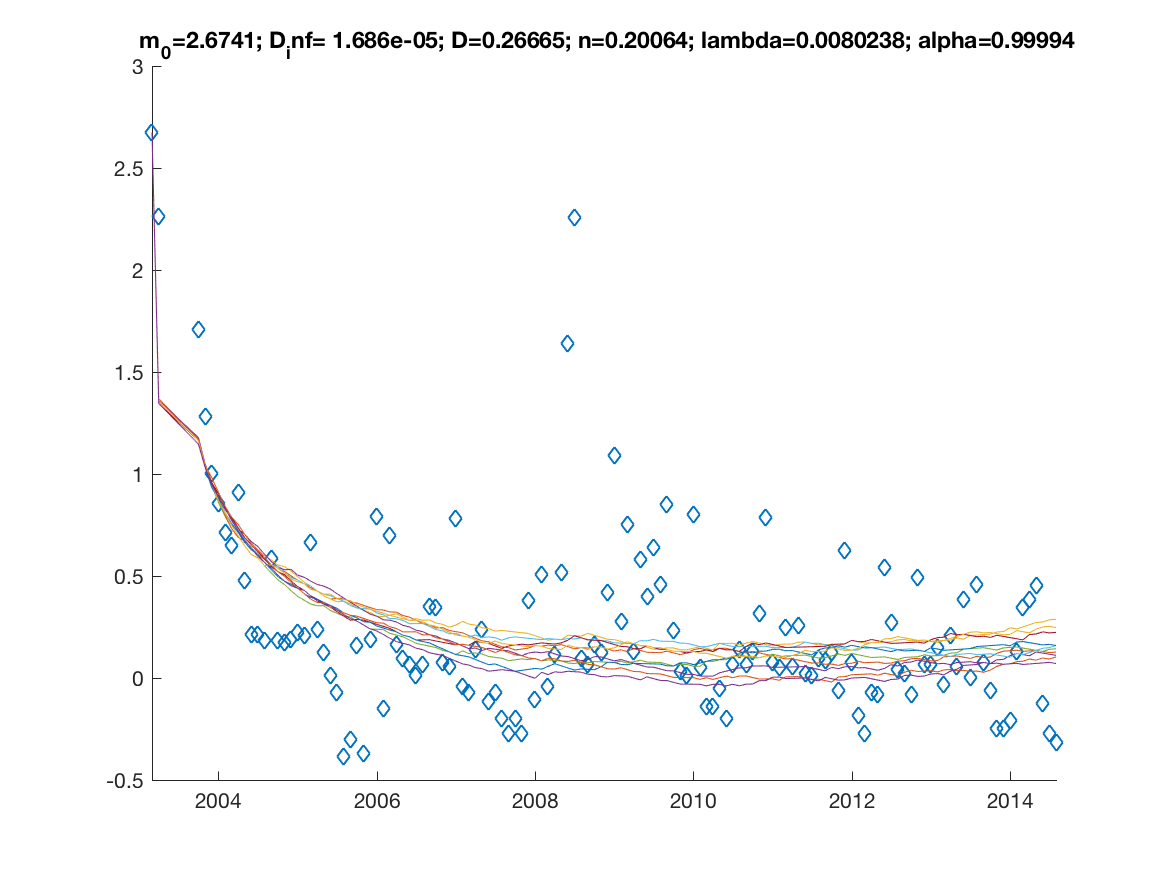
\includegraphics[width=0.9\textwidth  ]{BBplot_641} 
\end{center}
\end{figure}				
\end{frame}	

\section{3. Summary}
\begin{frame}
	\frametitle{Summary}
	\framesubtitle{Future Work}
	\justifying
\begin{itemize}
\item Improve the fit of uncertainty in the model for instance by combining Poisson and Brownian Motions.
		\item Find the spatial correlation between the gas production of wells in a region of interest, and use the correlation to forecast the performance of a new site based on the old wells around it.
		\item Relate the gas production forecast to the energy market forecast to calculate the profit in the future.
		\end{itemize}		
\end{frame}	

\begin{frame}	

\centering
{\Huge {\Huge Thank You!}}

\end{frame}
	
\end{document}	